\documentclass[10pt,a4paper]{article}
\usepackage[margin=2cm,headheight=15pt]{geometry}
\usepackage[T1]{fontenc}\usepackage{lmodern}\usepackage{CJKutf8}
\usepackage{amsmath,amssymb,booktabs,tabularx,array,float}
\usepackage{tikz,pgfplots}\usetikzlibrary{positioning,arrows.meta}\pgfplotsset{compat=1.18}
\usepackage{xcolor}\definecolor{accent}{HTML}{174C63}\definecolor{pale}{HTML}{EEF4F7}
\usepackage[unicode]{hyperref}\hypersetup{colorlinks=true,urlcolor=accent,linkcolor=accent}
\usepackage{fancyhdr}\pagestyle{fancy}\fancyhf{}\fancyhead[L]{KuaiRand | 第一周技术报告}\fancyhead[R]{2026 年 10 月}\fancyfoot[C]{\thepage}
\renewcommand{\headrulewidth}{.3pt}\renewcommand{\arraystretch}{1.3}
\setlength{\parindent}{0pt}\setlength{\parskip}{.55em}\setlength{\emergencystretch}{2em}\linespread{1.16}
\newcolumntype{Y}{>{\raggedright\arraybackslash}X}
\newcommand{\note}[1]{\par\smallskip\noindent\colorbox{pale}{\parbox{\dimexpr\linewidth-2\fboxsep}{\small #1}}\par\smallskip}
\begin{document}\begin{CJK*}{UTF8}{gbsn}
\renewcommand{\refname}{参考资料}\renewcommand{\tablename}{表}\renewcommand{\figurename}{图}
{\color{accent}\LARGE\bfseries KuaiRand 第一周技术报告}\par
{\large Pure 数据集上的双塔召回基线}\par
\textcolor{gray}{实验日期：2026 年 10 月 12 日\quad 数据协议：completion-time-v1}

\note{\textbf{核心结论：}数据审计、两组训练、向量导出、精确检索和受控 GPU 恢复验证已经跑通。热门基线 Recall@100 为 27.078\%，Basic 为 2.030\%，Enhanced 为 1.929\%。工程产物齐全，但当前双塔尚未体现个性化收益。}

\section{任务与数据范围}
我们研究的是\textbf{长观看导向的候选召回}：给定某个用户在某个时间点的上下文，从当时符合资格的视频中推荐前 100 个。模型输出排序分数，不输出经过校准的长观看概率。

监督标签直接使用官方 \texttt{long\_view}。视频不超过 18 秒时，观看达到视频时长算正反馈；更长的视频观看达到 18 秒算正反馈。训练只使用 \texttt{is\_random=0} 且 \texttt{long\_view=1} 的记录。非随机曝光指原推荐系统正常选择的视频；随机曝光来自数据集的随机干预机制，两者不能混为一谈。

\subsection{Pure 与完整数据集有什么区别？}
\begin{table}[H]\centering\small
\begin{tabularx}{\linewidth}{lrrY}\toprule
官方版本 & 用户数 & 视频规模 & 保留方式\\\midrule
KuaiRand-27K & 27,285 & 约 3,204 万 & 完整发布版本，保留这些用户在采集期的广泛行为记录。\\
KuaiRand-1K & 1,000 & 约 437 万 & 从 27K 随机抽取用户，保留这些用户的相关记录。\\
KuaiRand-Pure & 27,285 & 7,583 & 只保留固定候选池内视频的交互；删除池外视频记录。\\\bottomrule
\end{tabularx}\caption{官方版本口径，区别于下表中我们切分、去重后的实验规模。}\end{table}
Pure 不是“更干净的全量数据”，也不是只含随机曝光：它同时含常规曝光与随机曝光。官方常规曝光部分涉及 7,551 个视频，完整候选池为 7,583 个。\textbf{它主要缩减视频范围，而非用户范围；用户行为序列因此不完整。}本阶段用它验证闭环，不能据此判断长序列建模在完整 27K 上的效果。官方建议严格序列研究优先使用 27K 或 1K。\cite{dataset}

\subsection{本次实验实际规模}
\begin{table}[H]\centering\small
\begin{tabular}{lrrrr}\toprule
窗口 & 非随机曝光 & 长观看正反馈 & 正反馈比例 & 用户数\\\midrule
历史预热 & 886,326 & 297,920 & 33.61\% & 25,185\\
训练 & 363,643 & 124,255 & 34.17\% & 25,769\\
验证 & 94,578 & 30,589 & 32.34\% & 20,565\\\bottomrule
\end{tabular}\caption{精确整行去重后的规模；候选库共 7,583 个视频。测试集未参与本报告。}\end{table}
训练期正反馈集中在热门视频：前 100 个视频占训练正反馈的 26.83\%。这使热门计数成为必须比较的基线。

\clearpage
\section{数据处理与实际输入}
\subsection{时间切分与泄漏控制}
以 Unix 时间戳定义 UTC 窗口：4 月 15 日之前用于历史预热；4 月 15 日至 29 日之前训练；4 月 29 日至 5 月 4 日之前验证。测试集封存。去除 20,624 条所有原始字段完全相同的重复记录，保留真实重复观看。

历史反馈必须满足
\[
 t_{\mathrm{available}}=t_{\mathrm{request}}+\texttt{play\_time\_ms}
 <t_{\mathrm{current}}.
\]
因此，同一毫秒完成的观看不能进入当前请求历史。相较于只检查请求时间先后的做法，修正了 1,038 条历史。原始数据没有反馈入库时间，这只是保守的播放结束代理，不能声称还原了真实线上可用时刻。

原始日期与时间戳换算存在不一致，因此切分与周期特征统一使用显式 UTC 协议。类别词表只在训练范围拟合并冻结，未知类别使用索引 0；验证与测试不参与拟合。

\subsection{真正进入模型的特征}
\begin{table}[H]\centering\small
\begin{tabularx}{\linewidth}{p{2.4cm}p{3.5cm}Y}\toprule
输入 & 实际原始值示例 & 编码与维度\\\midrule
用户 ID\newline\texttt{user\_id} & 20853、8286 & 训练词表索引，32 维 embedding；未知用户索引 0。\\
场景\newline\texttt{tab} & 0、1、4；范围 0--14 & 类别索引，8 维 embedding。\\
请求时间\newline\texttt{time\_ms} & 1649475963278 毫秒 & UTC 日、周周期的正弦与余弦，共 4 维。\\
正反馈历史 & 最近最多 50 次已可用的视频 ID & 每个视频编码为 64 维；按 mask 求均值，得到 64 维。仅 Enhanced 使用。\\
历史 mask & 长度 50 的有效位标记 & 历史左侧补 $-1$；padding 不参与均值；空历史输出零向量。\\
物品 ID\newline\texttt{item\_id} & 0、1；原始 ID 0 编码为索引 1 & 训练词表索引，8 维 embedding；最终物品向量为 64 维。\\\bottomrule
\end{tabularx}\caption{Basic 和 Enhanced 共享 ID-only 物品塔；差别是用户塔是否加入历史。}\end{table}
请求时间示例经过周期编码约为 $(0.834,\,0.552,\,-0.997,\,-0.083)$。这些数值描述周期位置，不是标准化后的年份或日期。训练期未出现、但位于合法候选库中的物品也映射到未知类别。

\subsection{本次没有使用的字段}
作者、类型、标签、音乐、可见状态、视频时长与分辨率等物品属性来自无历史版本的元数据快照，无法证明在请求时可用，故不进入正式模型。\texttt{upload\_dt} 只用于候选资格：日期粒度为天的视频，从上传次日 UTC 零点起可推荐；资格信息缺失则排除。

标签、随机标记、请求 ID 和 split 用于过滤或评估，不作为模型输入。已有处理包括字段统一、切分和元数据准备；本阶段补充了整行去重、反馈完成时间历史、训练词表审计，以及活跃度、热门集中度、历史长度、缺失和未知类别统计。

\clearpage
\section{模型、损失与训练配置}
\subsection{两组架构}
\begin{figure}[H]\centering
\begin{minipage}[t]{.47\linewidth}\centering\textbf{用户塔}\par\medskip
\begin{tikzpicture}[node distance=5mm,box/.style={draw=accent,fill=pale,rounded corners=2pt,align=center,text width=6.2cm,minimum height=9mm,font=\small},>=Stealth]
\node[box] (a) {用户 ID 32 + 场景 8 + 时间 4};
\node[box,below=of a] (b) {Basic：44 维\\Enhanced：44 + 历史 64 = 108 维};
\node[box,below=of b] (c) {MLP：$44/108\to128\to64\to64$\\中间层 ReLU};
\node[box,below=of c] (d) {L2 归一化，输出 64 维};
\draw[->](a)--(b);\draw[->](b)--(c);\draw[->](c)--(d);
\end{tikzpicture}
\end{minipage}\hfill
\begin{minipage}[t]{.47\linewidth}\centering\textbf{物品塔（两组相同）}\par\medskip
\begin{tikzpicture}[node distance=5mm,box/.style={draw=accent,fill=pale,rounded corners=2pt,align=center,text width=6.2cm,minimum height=9mm,font=\small},>=Stealth]
\node[box] (a) {原始视频 ID};
\node[box,below=of a] (b) {冻结词表 $\to$ 8 维 embedding};
\node[box,below=of b] (c) {MLP：$8\to64\to64$\\中间层 ReLU};
\node[box,below=of c] (d) {L2 归一化，输出 64 维};
\draw[->](a)--(b);\draw[->](b)--(c);\draw[->](c)--(d);
\end{tikzpicture}
\end{minipage}
\caption{Enhanced 增强的是用户历史，没有加入未经时间审计的物品内容。历史与目标共享物品塔参数。}
\end{figure}
用户、物品的匹配分为归一化向量点积：
\[
 s(u,i)=f_\theta(u,t,h)^\top g_\phi(i),\qquad
 \|f_\theta\|_2=\|g_\phi\|_2=1.
\]

\subsection{监督信号与损失}
每个 batch 包含 $B$ 条真实长观看用户--物品对，对角线为正目标。设 $D_i$ 是与第 $i$ 个目标视频重复的非对角位置，则
\[
\mathcal L=-\frac1B\sum_{i=1}^{B}
\log\frac{\exp(s(u_i,i_i)/\tau)}{\sum_{j\notin D_i}\exp(s(u_i,i_j)/\tau)},\qquad \tau=0.1.
\]
重复目标位置被屏蔽，但对角线保留。其余物品是批内采样的比较对象，\textbf{并非已知的用户负反馈}，可能包含用户也喜欢的视频。当前没有采样频率修正。

\subsection{冻结的公平比较配置}
\begin{table}[H]\centering\small
\begin{tabularx}{\linewidth}{lYlY}\toprule
项目 & 设置 & 项目 & 设置\\\midrule
随机种子 & 42，同一打乱顺序 & Batch / Epoch & 256 / 1\\
优化器 & Adam，$\beta=(0.9,0.999)$ & 学习率 & 0.001\\
Weight decay & 0 & Temperature & 0.1\\
Dropout / BN & 0 / 关闭 & 输出维度 & 64，L2 归一化\\
设备 & A100-SXM4-40GB，CUDA AMP & 运行环境 & Python 3.11.15；PyTorch 2.14.1+cu130\\\bottomrule
\end{tabularx}\caption{两组使用相同数据、预算与优化设置；本次未进行超参数搜索。}\end{table}

\clearpage
\section{训练结果与恢复验证}
\begin{table}[H]\centering\small
\begin{tabular}{lrrrrr}\toprule
模型 & 消费样本 & 更新步数 & 验证 loss & Step+wait（秒） & 峰值显存（MiB）\\\midrule
Basic & 124,255 & 486 & 5.535129 & 7.243 & 83.85\\
Enhanced & 124,255 & 486 & 5.530827 & 8.636 & 97.61\\\bottomrule
\end{tabular}\caption{耗时为日志中的读取等待与训练 step 之和，不含完整验证、checkpoint 保存和编排；显存为 PyTorch allocated 峰值。}\end{table}
\begin{figure}[H]\centering
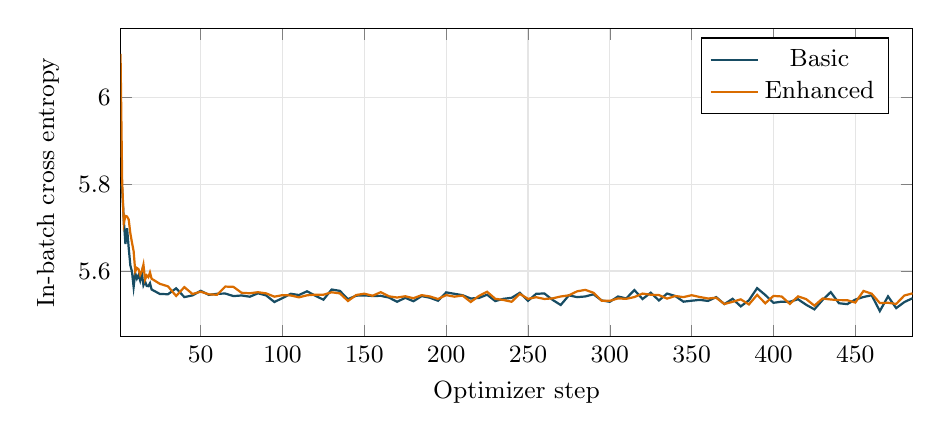
\begin{tikzpicture}\begin{axis}[width=.96\linewidth,height=5.5cm,xlabel={Optimizer step},ylabel={In-batch cross entropy},grid=major,grid style={gray!20},legend pos=north east,tick label style={font=\small},label style={font=\small},legend style={font=\small},xmin=1,xmax=485]
\addplot[color=accent,thick] coordinates {(1,5.8004608) (2,5.7875061) (3,5.7169495) (4,5.6619415) (5,5.6988068) (6,5.6531525) (7,5.6130524) (8,5.5986023) (9,5.5633240) (10,5.5949554) (11,5.5827026) (12,5.5905304) (13,5.5780640) (14,5.5959015) (15,5.5672760) (16,5.5760803) (17,5.5656281) (18,5.5650482) (19,5.5719147) (20,5.5573730) (25,5.5471802) (30,5.5464478) (35,5.5601349) (40,5.5399170) (45,5.5437775) (50,5.5543671) (55,5.5450134) (60,5.5474854) (65,5.5480957) (70,5.5421753) (75,5.5436249) (80,5.5407562) (85,5.5486603) (90,5.5437317) (95,5.5286102) (100,5.5375366) (105,5.5475311) (110,5.5446167) (115,5.5532379) (120,5.5430756) (125,5.5338898) (130,5.5573578) (135,5.5542755) (140,5.5351562) (145,5.5431213) (150,5.5438232) (155,5.5423737) (160,5.5427551) (165,5.5388336) (170,5.5291138) (175,5.5382538) (180,5.5303345) (185,5.5421753) (190,5.5384827) (195,5.5314789) (200,5.5507507) (205,5.5474854) (210,5.5442963) (215,5.5366058) (220,5.5379181) (225,5.5453644) (230,5.5307159) (235,5.5359039) (240,5.5382385) (245,5.5498047) (250,5.5312805) (255,5.5474396) (260,5.5482635) (265,5.5335083) (270,5.5216980) (275,5.5439301) (280,5.5397797) (285,5.5413208) (290,5.5463257) (295,5.5322113) (300,5.5290833) (305,5.5413055) (310,5.5367126) (315,5.5561218) (320,5.5354614) (325,5.5499725) (330,5.5321655) (335,5.5480499) (340,5.5423584) (345,5.5293121) (350,5.5315247) (355,5.5334930) (360,5.5310059) (365,5.5398254) (370,5.5237732) (375,5.5359039) (380,5.5184784) (385,5.5324402) (390,5.5605621) (395,5.5446625) (400,5.5267181) (405,5.5293427) (410,5.5290833) (415,5.5349426) (420,5.5221405) (425,5.5116272) (430,5.5331573) (435,5.5513992) (440,5.5257492) (445,5.5236282) (450,5.5340881) (455,5.5400848) (460,5.5441132) (465,5.5077209) (470,5.5415497) (475,5.5144424) (480,5.5284729) (485,5.5372925)};\addlegendentry{Basic}
\addplot[color=orange!85!black,thick] coordinates {(1,6.1000748) (2,5.8072128) (3,5.7100372) (4,5.7269135) (5,5.7256470) (6,5.7185669) (7,5.6869049) (8,5.6656036) (9,5.6456757) (10,5.5991364) (11,5.6070251) (12,5.6041718) (13,5.5910797) (14,5.5993195) (15,5.6147461) (16,5.5803833) (17,5.5897980) (18,5.5856934) (19,5.5966492) (20,5.5821686) (25,5.5704803) (30,5.5646515) (35,5.5424652) (40,5.5628357) (45,5.5469666) (50,5.5523529) (55,5.5462189) (60,5.5452271) (65,5.5641327) (70,5.5634613) (75,5.5497589) (80,5.5487213) (85,5.5511780) (90,5.5484467) (95,5.5408173) (100,5.5444031) (105,5.5437012) (110,5.5393372) (115,5.5440674) (120,5.5454712) (125,5.5453491) (130,5.5509491) (135,5.5484924) (140,5.5309143) (145,5.5445862) (150,5.5477600) (155,5.5429077) (160,5.5511780) (165,5.5416870) (170,5.5388947) (175,5.5418091) (180,5.5372620) (185,5.5443573) (190,5.5414124) (195,5.5355072) (200,5.5444336) (205,5.5408936) (210,5.5434418) (215,5.5286102) (220,5.5425720) (225,5.5521545) (230,5.5359650) (235,5.5332184) (240,5.5290985) (245,5.5472412) (250,5.5358582) (255,5.5395660) (260,5.5355377) (265,5.5369720) (270,5.5412750) (275,5.5439148) (280,5.5531616) (285,5.5565186) (290,5.5498810) (295,5.5316315) (300,5.5312042) (305,5.5368652) (310,5.5358582) (315,5.5399475) (320,5.5479736) (325,5.5453033) (330,5.5445404) (335,5.5363770) (340,5.5424347) (345,5.5398560) (350,5.5442047) (355,5.5400543) (360,5.5366364) (365,5.5383911) (370,5.5239716) (375,5.5289459) (380,5.5347137) (385,5.5229187) (390,5.5449829) (395,5.5256042) (400,5.5425873) (405,5.5412903) (410,5.5241394) (415,5.5414581) (420,5.5351715) (425,5.5202332) (430,5.5365906) (435,5.5343323) (440,5.5328979) (445,5.5327911) (450,5.5272675) (455,5.5539703) (460,5.5477905) (465,5.5261688) (470,5.5267334) (475,5.5241547) (480,5.5435486) (485,5.5485077)};\addlegendentry{Enhanced}
\end{axis}\end{tikzpicture}\caption{实际训练 loss；前 20 步逐步展示，之后每 5 步取一个日志点。只画完整 batch，避免尾批造成误导。}\end{figure}
\textbf{尾批骤降的原因：}前 485 批各 256 条，最后一批为 95 条。均匀打分的参考交叉熵会由 $\ln256=5.545$ 降至 $\ln95=4.554$，并受重复目标屏蔽影响。实际尾批 loss 为 4.535（Basic）和 4.538（Enhanced），不能当作突然学好了。

相同验证批次与重复屏蔽下，均匀打分参考 loss 约为 5.540678。两组验证 loss 仅略低于此值，与较弱的召回效果一致；批内 loss 稳定不等于全候选检索有效。

\subsection{导出与恢复}
两组各导出 7,583 个归一化 64 维物品向量，候选 ID、维度、有限值、单位范数和 checkpoint 绑定均通过检查。Enhanced 在第 25 步保存，恢复后最终消费 124,255 条样本、完成 486 步。模型、Adam、AMP、随机状态与游标均与连续训练\textbf{完全一致}。

这验证了\textbf{同一环境中的受控保存与恢复}，尚未验证 Colab 断线或重建 runtime 后恢复。checkpoint 文件 hash 不同可以来自运行元信息与序列化差异；验收比较的是训练状态。

\clearpage
\section{评估协议与结果}
\subsection{每条请求如何判断命中？}
取验证期所有非随机长观看记录。每条记录给出“哪个用户、什么时间、实际长观看了哪个视频”，这个视频就是该条请求的唯一正目标。

热门基线按\textbf{训练期非随机长观看次数}给视频排序；双塔按该请求用户向量与物品向量的点积排序。两者生成推荐时都不知道当前目标标签，使用相同候选库与资格规则；同分按原始视频 ID 升序。允许推荐历史看过的视频，参数在验证期不更新。

\note{\textbf{分子：}实际目标进入该请求 Top-100 的请求数。\quad
\textbf{分母：}全部 30,589 条验证请求。\quad
100 是每次推荐的数量，不是分母。同一用户多次观看分别评估，不合并视频去重。}
令 $r_q$ 为第 $q$ 条请求的目标排名；未进入榜单或不具备候选资格时视为未命中：
\[
\mathrm{Recall@100}=\frac{\sum_{q=1}^{Q}\mathbf1[r_q\le100]}{Q},
\qquad Q=30,589.
\]
\[
\mathrm{NDCG@100}=\frac1Q\sum_{q=1}^{Q}
\frac{\mathbf1[r_q\le100]}{\log_2(r_q+1)}.
\]
Recall 只看是否进入前 100；NDCG 同时看位置，排第 1 得 1 分，排第 10 约得 0.289 分，排第 100 约得 0.150 分。本指标按请求平均，活跃用户权重更大；尚未计算每个用户等权的平均命中率。

\subsection{三组在同一协议上的比较}
\begin{table}[H]\centering
\begin{tabular}{lrrrr}\toprule
模型 & 命中请求数 & Recall@100 & NDCG@100 & 目标覆盖率\\\midrule
\textbf{热门基线} & \textbf{8,283} & \textbf{27.078\%} & \textbf{0.069607} & 100\%\\
Basic 双塔 & 621 & 2.030\% & 0.005489 & 100\%\\
Enhanced 双塔 & 590 & 1.929\% & 0.004112 & 100\%\\\bottomrule
\end{tabular}\caption{已从逐请求预测独立复算命中数与 NDCG，并核对冻结请求身份与产物版本。}\end{table}
三组每次均返回 100 个不重复且符合资格的视频；目标覆盖率为 100\%，因此条件指标与端到端指标相同。热门计数只使用训练期标签，并未使用验证答案，不属于标签泄漏。

\textbf{实验结论：}热门明显领先两组双塔；Enhanced 少命中 31 条请求，没有证明平均历史带来了收益。当前只有 seed 42、1 epoch，不能把两组的小差异解释成稳定优势或劣势。验证来自原推荐策略的曝光，结果也不能直接等同线上收益。

\clearpage
\section{成本、限制与下一周安排}
\subsection{评估成本与覆盖}
用户编码在 GPU，精确点积与排序在 CPU。分块检索避免常驻完整请求 $\times$ 候选矩阵。下表使用 batch 256、排除 1 个预热 batch；包含特征组装、编码、必要的 GPU 到 CPU 传输与检索，不含初始模型和数据加载。
\begin{table}[H]\centering\small
\begin{tabular}{lrrrr}\toprule
模型 & 用户编码（秒） & 检索（秒） & Batch P50（秒） & Batch P95（秒）\\\midrule
热门 & 0.002474 & 13.566819 & 0.113596 & 0.116308\\
Basic & 0.426576 & 25.620920 & 0.207204 & 0.277423\\
Enhanced & 0.565114 & 25.485775 & 0.208044 & 0.269540\\\bottomrule
\end{tabular}\caption{Colab 实测批量耗时，不是线上单请求延迟，也不是 GPU 检索性能。}\end{table}
验证请求中未知用户 1,213 条（3.965\%），空历史 456 条（1.491\%）。训练词表未收录的物品 ID 占候选库的 9.244\%，占验证正目标的 0.111\%；这些 ID 使用未知 embedding，但仍在合法候选库中，不等于目标缺失。

\subsection{解释边界}
Pure 删除池外观看，历史不完整；反馈完成时间和上传资格均依赖代理规则。物品内容没有可验证的历史版本，已从模型排除。只有一次短预算训练，未测多 seed、用户等权指标或上线效果。批内比较可能包含假负例和采样偏差。\textbf{目前没有证据把弱效果归因于某一个代码错误或单一超参数。}

\subsection{下一周优先任务}
\begin{enumerate}
\item 在冻结验证协议下，先增加训练轮数并逐轮评估 Recall/NDCG，判断是否充分学习；保持当前一轮结果作为基线，不同时修改所有参数。
\item 扩展到 27K，并冻结嵌套用户子集。比较基础、仅历史、仅物品增强、联合增强四组；物品增强必须先通过时间有效性审计。
\item 增加用户等权、长尾、冷启动和历史长度切片；补充多 seed 稳定性与新 runtime 恢复检查。
\item 再分别检验 item embedding 容量、学习率和采样修正，根据吞吐与内存确定扩展预算。封存测试集继续不参与选型。
\end{enumerate}

\subsection{复现入口与依据}
代码位于 \texttt{research/kuairand/}。执行版本为 \texttt{c29eb45}，Drive release 为 \texttt{week1-pure-completion-v1-001}。完整校验值和聚合结果见报告旁的 \texttt{report\_evidence.json} 与 \texttt{evidence/}；checkpoint、向量与逐请求数据留在私有 Drive，不在正文堆叠长 hash。

训练 run：Basic \texttt{5d0da236b294}；Enhanced \texttt{ce21055c8126}；恢复验收 \texttt{723f7c5b353e}。恢复 run 不是第三种模型。数据和模型使用既有流水线，未另建训练系统。

\begin{thebibliography}{9}\small
\bibitem{dataset} KuaiRand 官方数据版本与字段说明：\url{https://kuairand.com/}。
\bibitem{paper} Gao 等，KuaiRand，CIKM 2022：\url{https://arxiv.org/abs/2208.08696}。
\end{thebibliography}
\clearpage\end{CJK*}\end{document}
